%% Unit 4: Design Thinking & Customer Centricity
%% Included from main.tex via %% Unit 4: Design Thinking & Customer Centricity
%% Included from main.tex via %% Unit 4: Design Thinking & Customer Centricity
%% Included from main.tex via %% Unit 4: Design Thinking & Customer Centricity
%% Included from main.tex via \include{./units/unit4}
%% Requires the macros/colours defined in main.tex's preamble.

%==============================================================================
\section{Design Thinking \& Customer Centricity}
%==============================================================================
\unitdivider{IV}{Design Thinking \&\\Customer Centricity}{Experience, feedback \& re-creation}

\begin{frame}{Practical Customer Challenges}
  \accentrule\\[0.3em]
  \small
  Real customers face everyday frustrations that design thinking can solve:
  \begin{columns}[T]
    \begin{column}{0.5\textwidth}
      \begin{itemize}\small
        \item Products that are \kwc{hard to assemble} or use.
        \item Confusing instructions \& interfaces.
        \item Poor \kwc{ergonomics} causing discomfort.
      \end{itemize}
    \end{column}
    \begin{column}{0.5\textwidth}
      \begin{itemize}\small
        \item Long waits and clunky service.
        \item Features nobody asked for.
        \item A gap between the \emph{promise} and the \emph{experience}.
      \end{itemize}
    \end{column}
  \end{columns}
  \vspace{0.4em}
  \begin{block}{Design thinking to the rescue}\scriptsize
    By empathising with customers we uncover these pains and re-design the
    product experience around them.
  \end{block}
\end{frame}

\begin{frame}{Parameters of Product Experience}
  \begin{columns}[c]
    \begin{column}{0.55\textwidth}
      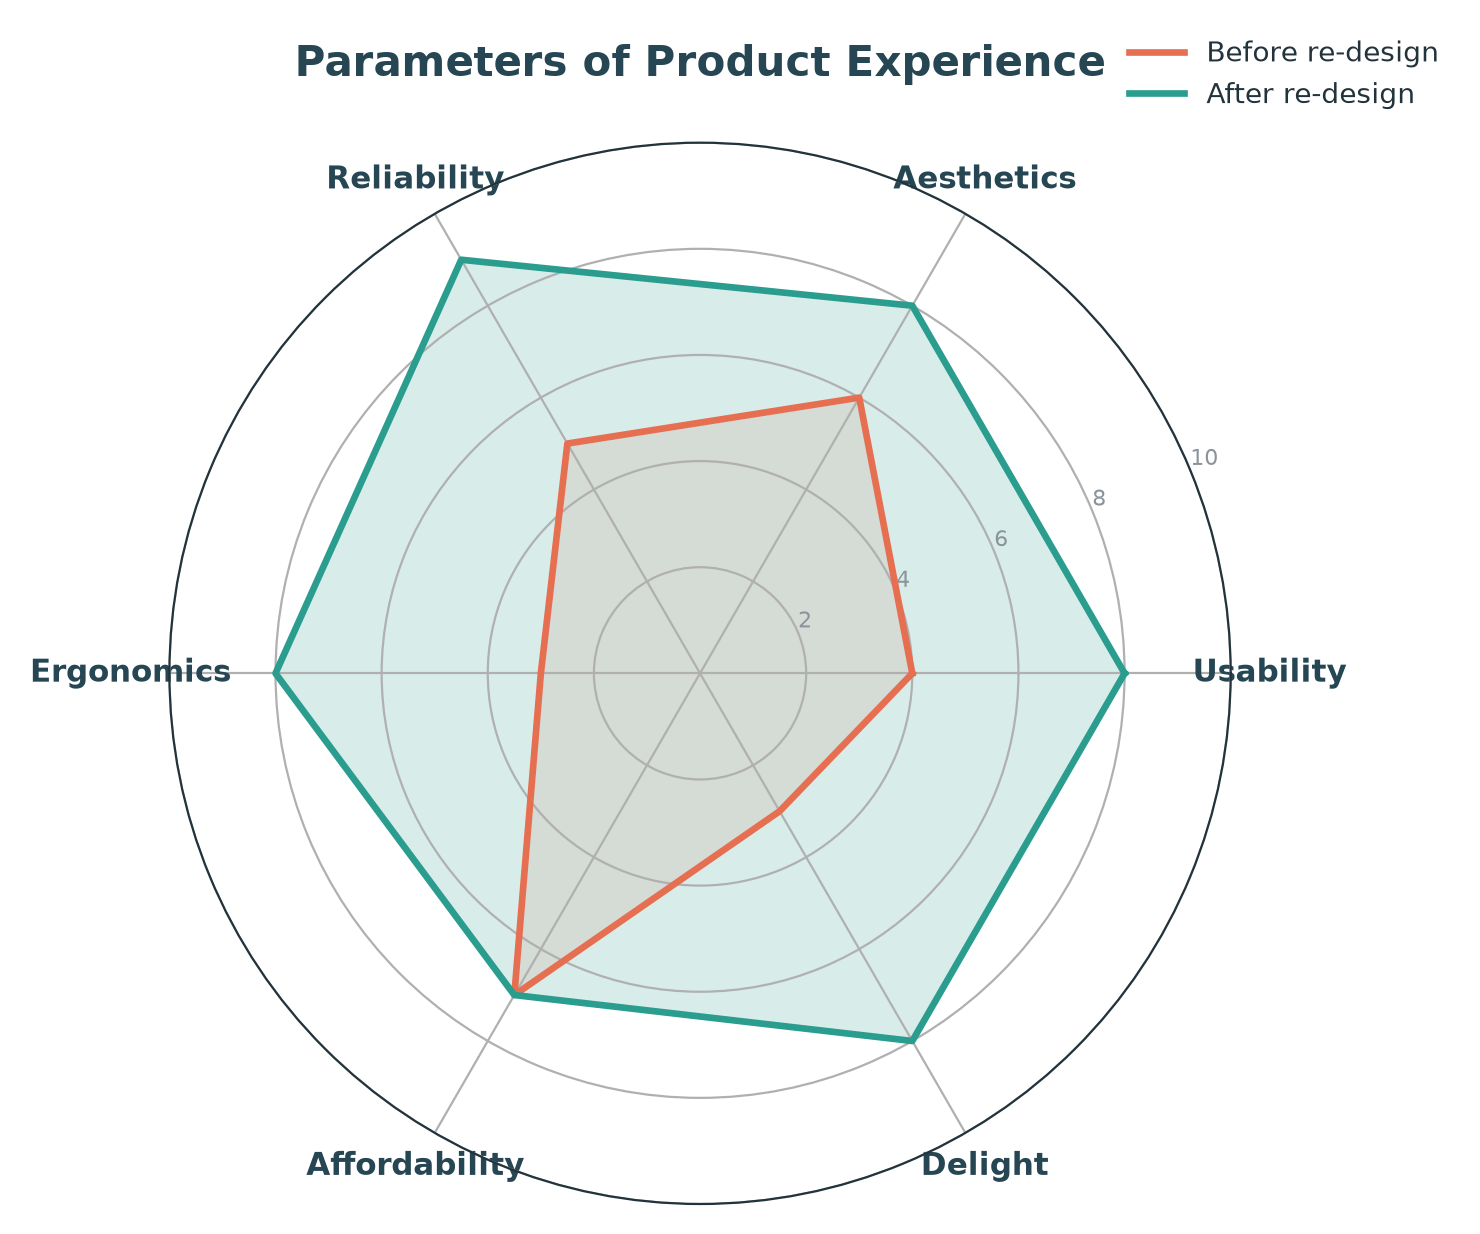
\includegraphics[width=\linewidth]{figures/cx_radar.png}
    \end{column}
    \begin{column}{0.45\textwidth}\scriptsize
      Product experience is multi-dimensional:
      \begin{itemize}\scriptsize
        \item \kwt{Usability} \& \kwt{Reliability}
        \item \kwt{Aesthetics} \& \kwt{Ergonomics}
        \item \kwt{Affordability} \& \kwt{Delight}
      \end{itemize}
      \vspace{0.3em}
      Thoughtful re-design lifts every axis — turning a merely functional
      product into one customers \emph{love}.
    \end{column}
  \end{columns}
\end{frame}

\begin{frame}{Aligning Customer Expectations}
  \begin{columns}[c]
    \begin{column}{0.55\textwidth}
      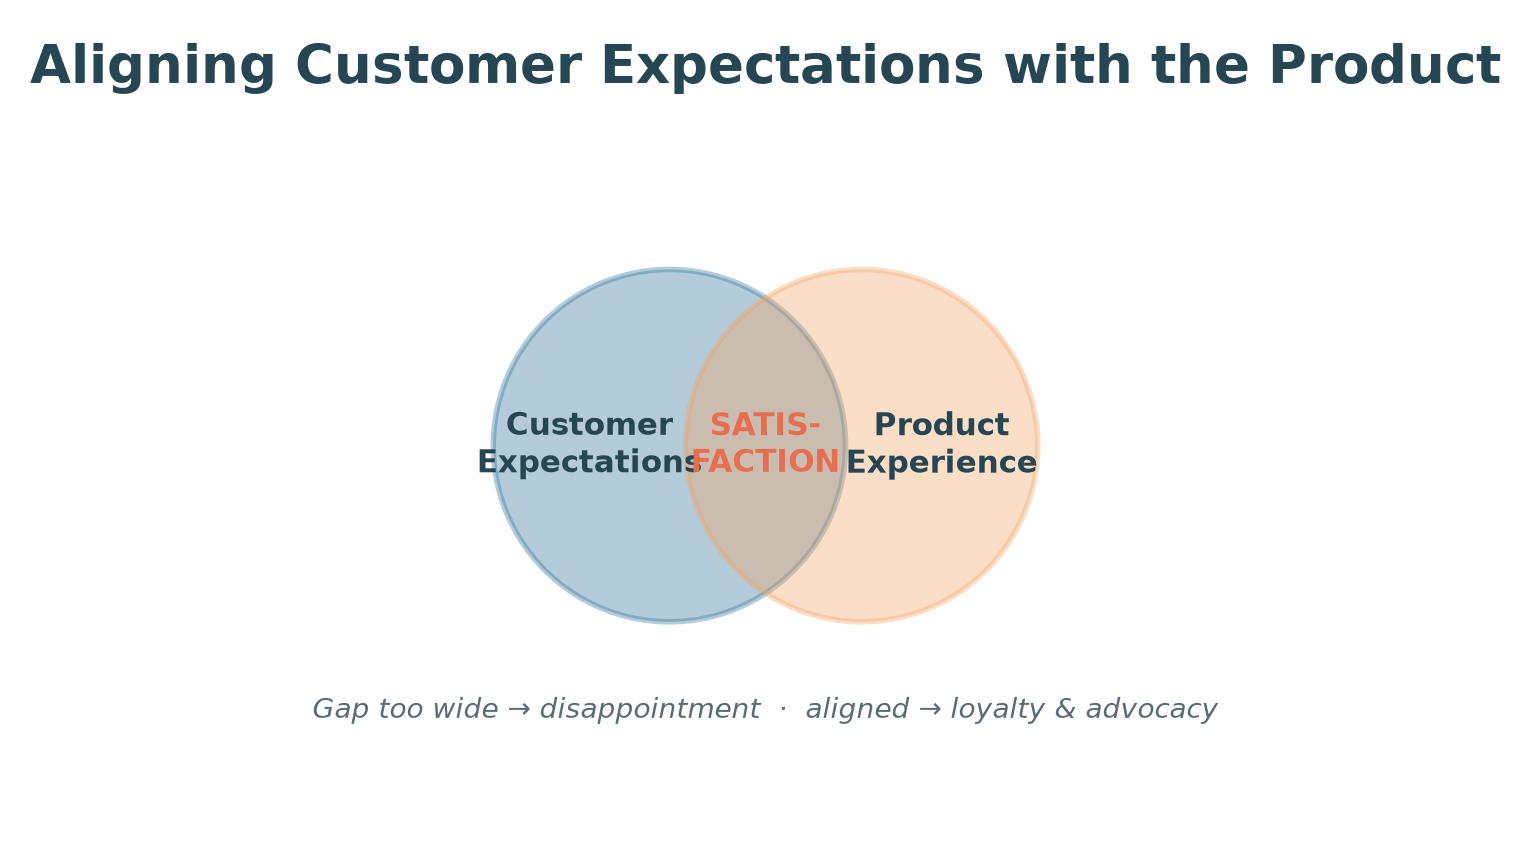
\includegraphics[width=\linewidth]{figures/expectation_alignment.png}
    \end{column}
    \begin{column}{0.45\textwidth}\scriptsize
      \kw{Satisfaction} lives where \emph{expectations} meet \emph{experience}.
      \begin{itemize}\scriptsize
        \item Gap too wide $\to$ disappointment.
        \item Well aligned $\to$ loyalty \& advocacy.
      \end{itemize}
      \vspace{0.3em}
      Manage expectations honestly \emph{and} raise the experience to close
      the gap.
    \end{column}
  \end{columns}
\end{frame}

\begin{frame}{Feedback, Re-Design \& Re-Create}
  \begin{columns}[c]
    \begin{column}{0.52\textwidth}
      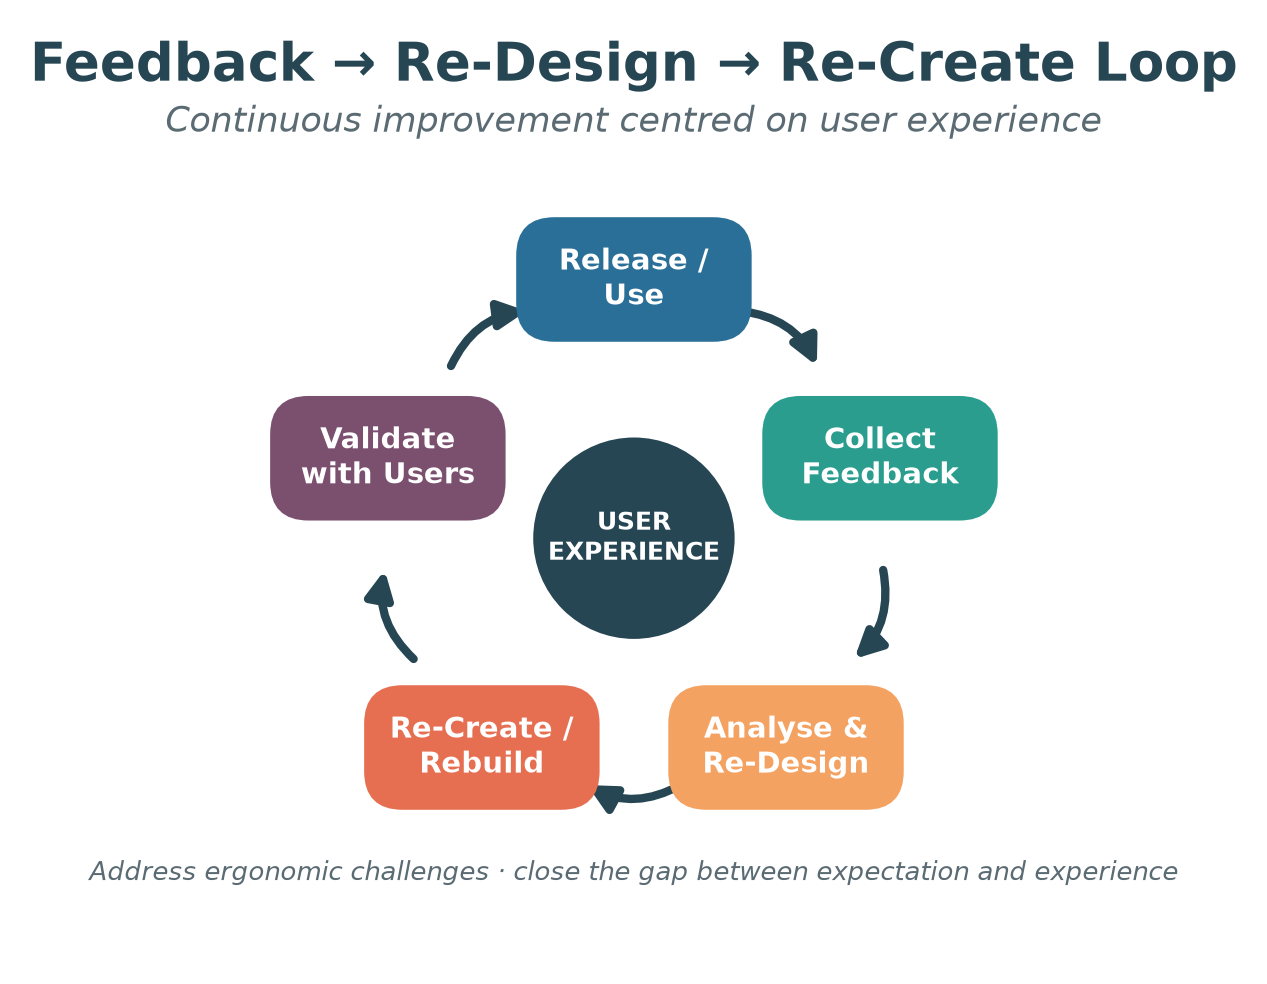
\includegraphics[width=\linewidth]{figures/feedback_loop.png}
    \end{column}
    \begin{column}{0.48\textwidth}\scriptsize
      The \kw{feedback loop} keeps a product improving:
      \begin{enumerate}\scriptsize
        \item Release \& use.
        \item Collect feedback.
        \item Analyse \& re-design.
        \item Re-create / rebuild.
        \item Validate with users.
      \end{enumerate}
      \vspace{0.2em}
      Focus relentlessly on \kwt{user experience} and address ergonomic
      challenges each cycle.
    \end{column}
  \end{columns}
\end{frame}

\begin{frame}{User-Focused Design \& the Final Product}
  \accentrule\\[0.3em]
  \begin{columns}[T]
    \begin{column}{0.5\textwidth}\small
      \textbf{User-focused design}
      \begin{itemize}\small
        \item Design \emph{with} users, not just for them.
        \item Fit the product to the human — \kwt{ergonomics}.
        \item Test with real tasks in real contexts.
      \end{itemize}
    \end{column}
    \begin{column}{0.5\textwidth}\small
      \textbf{Toward the final product}
      \begin{itemize}\small
        \item Converge feedback into refinements.
        \item Validate safety, comfort \& usability.
        \item Ship — then keep listening.
      \end{itemize}
    \end{column}
  \end{columns}
  \vspace{0.3em}
  \begin{block}{Remember}\scriptsize
    A "final" product is really the \emph{best current version} — the loop
    never truly ends.
  \end{block}
\end{frame}

%% Requires the macros/colours defined in main.tex's preamble.

%==============================================================================
\section{Design Thinking \& Customer Centricity}
%==============================================================================
\unitdivider{IV}{Design Thinking \&\\Customer Centricity}{Experience, feedback \& re-creation}

\begin{frame}{Practical Customer Challenges}
  \accentrule\\[0.3em]
  \small
  Real customers face everyday frustrations that design thinking can solve:
  \begin{columns}[T]
    \begin{column}{0.5\textwidth}
      \begin{itemize}\small
        \item Products that are \kwc{hard to assemble} or use.
        \item Confusing instructions \& interfaces.
        \item Poor \kwc{ergonomics} causing discomfort.
      \end{itemize}
    \end{column}
    \begin{column}{0.5\textwidth}
      \begin{itemize}\small
        \item Long waits and clunky service.
        \item Features nobody asked for.
        \item A gap between the \emph{promise} and the \emph{experience}.
      \end{itemize}
    \end{column}
  \end{columns}
  \vspace{0.4em}
  \begin{block}{Design thinking to the rescue}\scriptsize
    By empathising with customers we uncover these pains and re-design the
    product experience around them.
  \end{block}
\end{frame}

\begin{frame}{Parameters of Product Experience}
  \begin{columns}[c]
    \begin{column}{0.55\textwidth}
      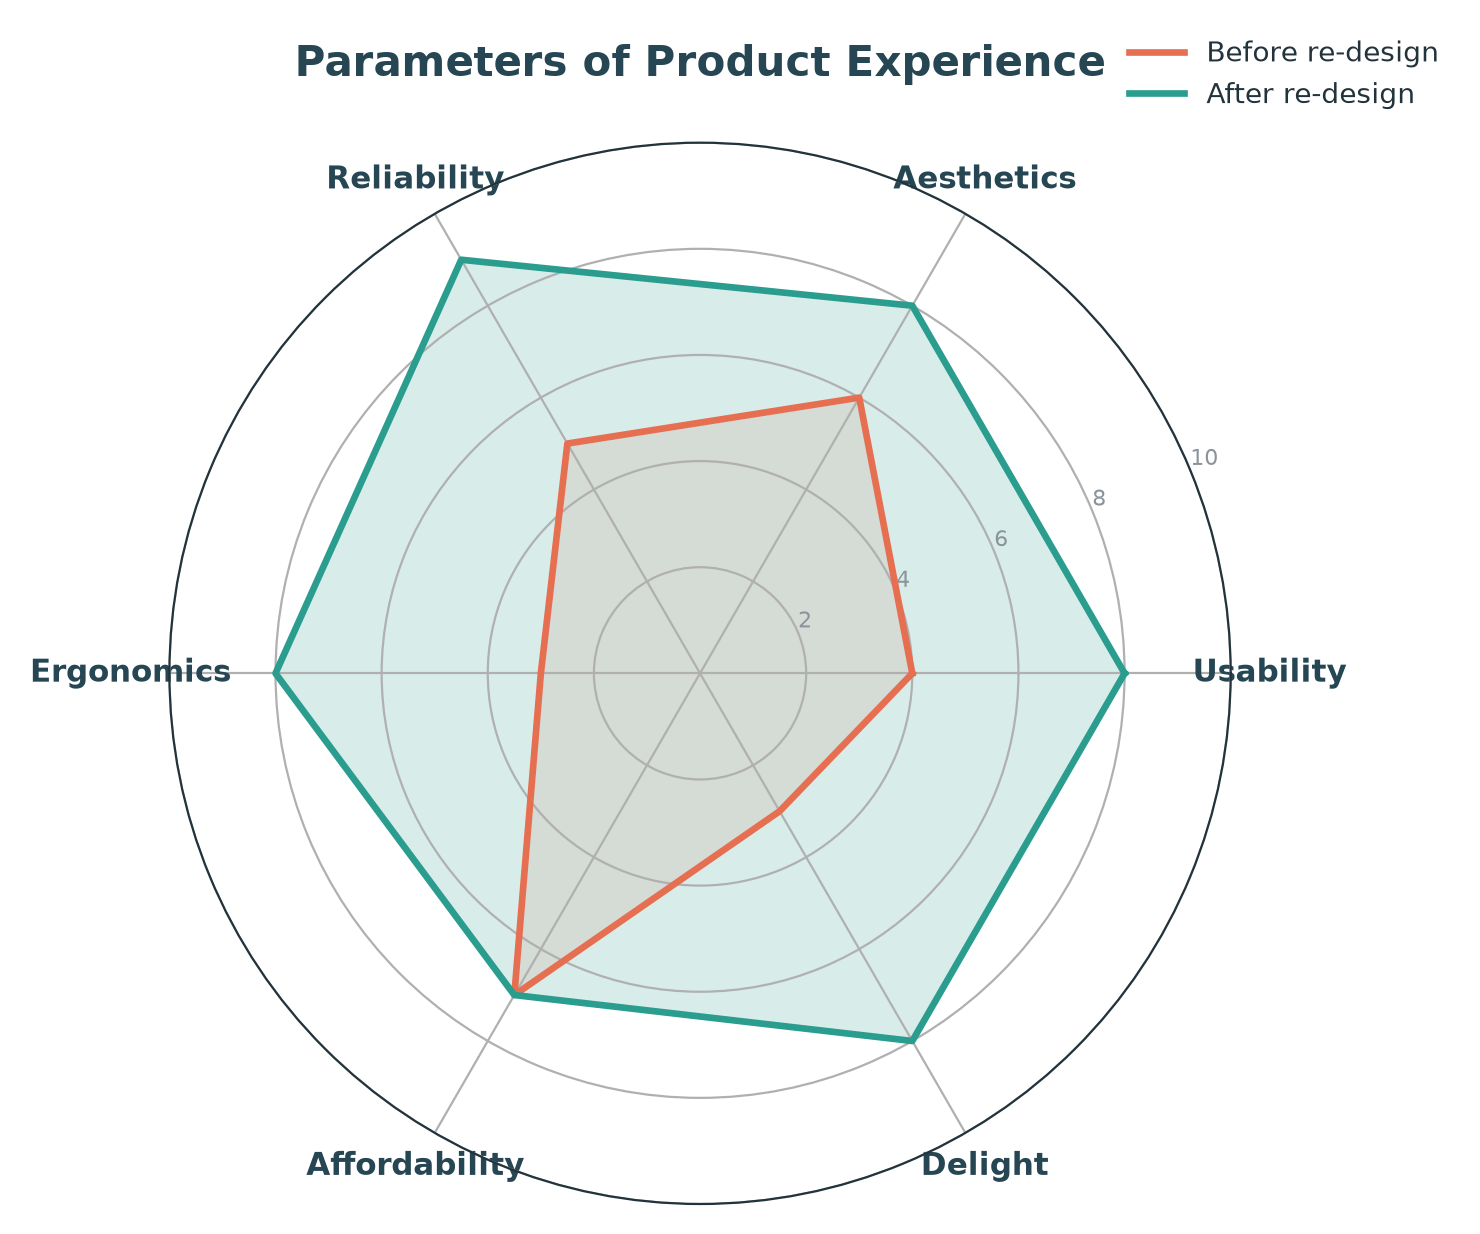
\includegraphics[width=\linewidth]{figures/cx_radar.png}
    \end{column}
    \begin{column}{0.45\textwidth}\scriptsize
      Product experience is multi-dimensional:
      \begin{itemize}\scriptsize
        \item \kwt{Usability} \& \kwt{Reliability}
        \item \kwt{Aesthetics} \& \kwt{Ergonomics}
        \item \kwt{Affordability} \& \kwt{Delight}
      \end{itemize}
      \vspace{0.3em}
      Thoughtful re-design lifts every axis — turning a merely functional
      product into one customers \emph{love}.
    \end{column}
  \end{columns}
\end{frame}

\begin{frame}{Aligning Customer Expectations}
  \begin{columns}[c]
    \begin{column}{0.55\textwidth}
      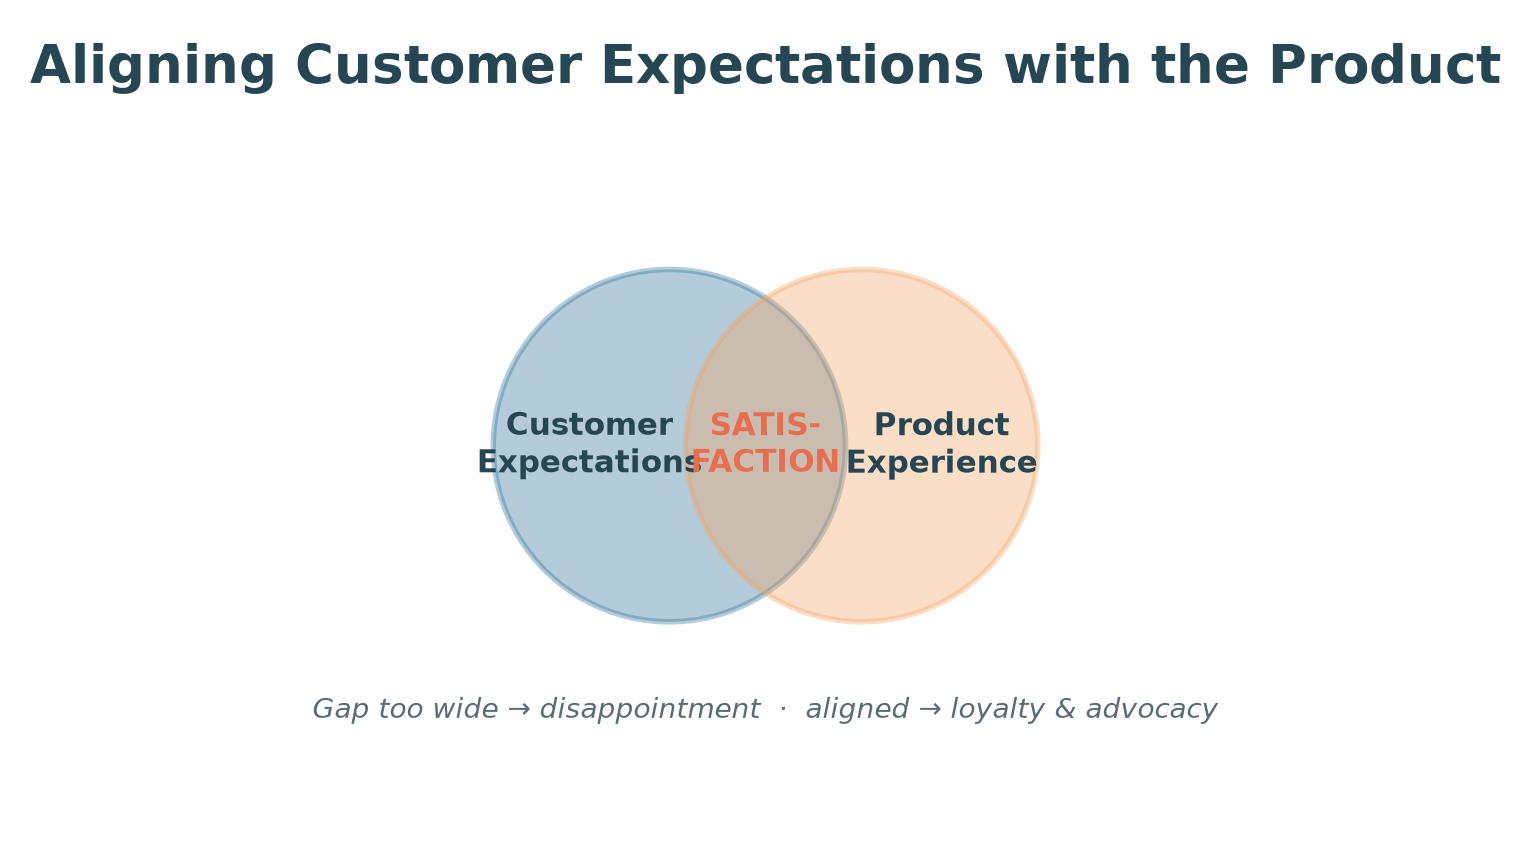
\includegraphics[width=\linewidth]{figures/expectation_alignment.png}
    \end{column}
    \begin{column}{0.45\textwidth}\scriptsize
      \kw{Satisfaction} lives where \emph{expectations} meet \emph{experience}.
      \begin{itemize}\scriptsize
        \item Gap too wide $\to$ disappointment.
        \item Well aligned $\to$ loyalty \& advocacy.
      \end{itemize}
      \vspace{0.3em}
      Manage expectations honestly \emph{and} raise the experience to close
      the gap.
    \end{column}
  \end{columns}
\end{frame}

\begin{frame}{Feedback, Re-Design \& Re-Create}
  \begin{columns}[c]
    \begin{column}{0.52\textwidth}
      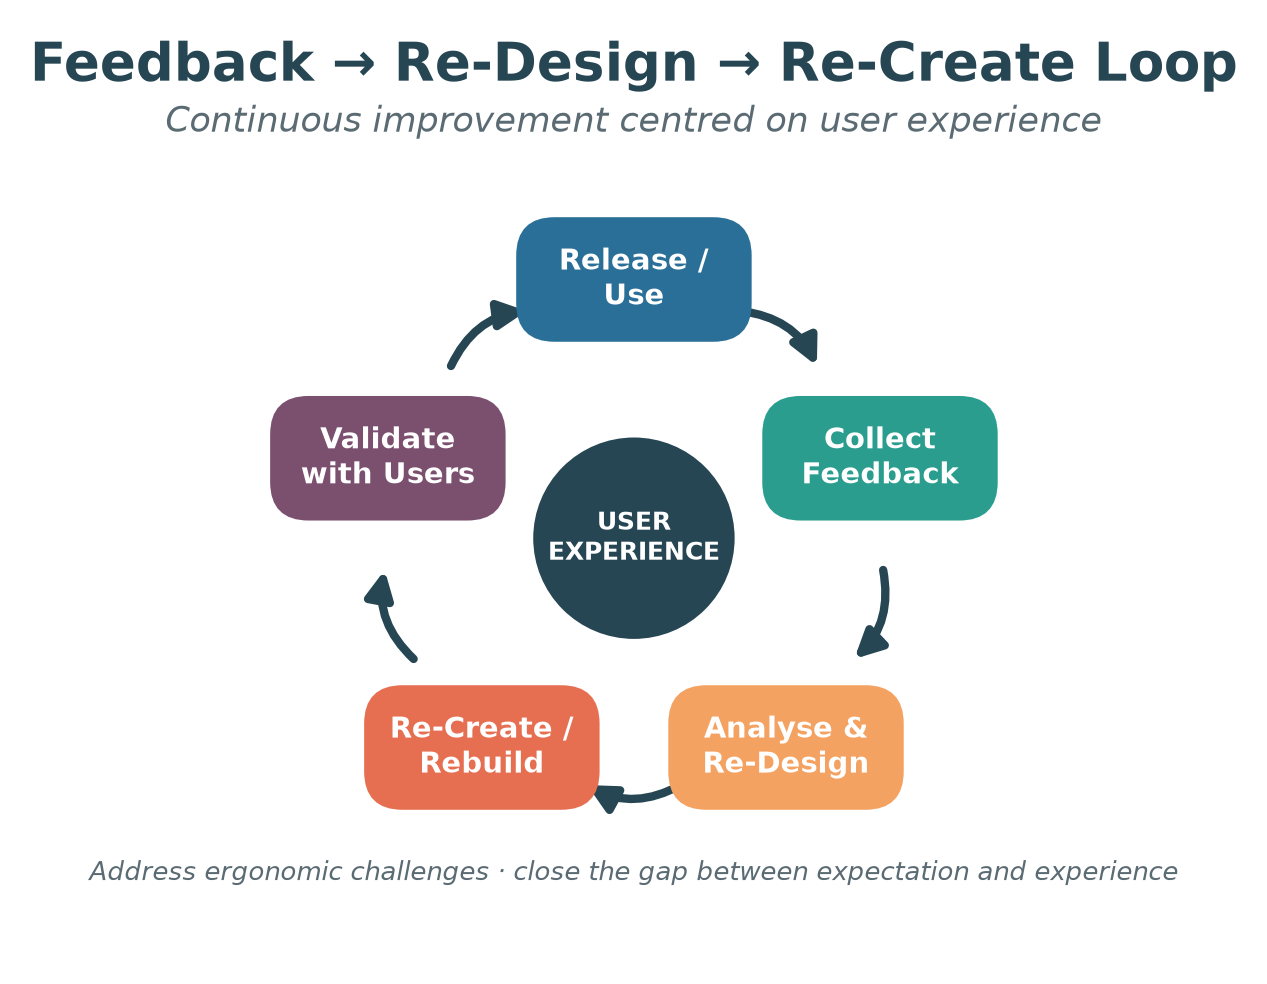
\includegraphics[width=\linewidth]{figures/feedback_loop.png}
    \end{column}
    \begin{column}{0.48\textwidth}\scriptsize
      The \kw{feedback loop} keeps a product improving:
      \begin{enumerate}\scriptsize
        \item Release \& use.
        \item Collect feedback.
        \item Analyse \& re-design.
        \item Re-create / rebuild.
        \item Validate with users.
      \end{enumerate}
      \vspace{0.2em}
      Focus relentlessly on \kwt{user experience} and address ergonomic
      challenges each cycle.
    \end{column}
  \end{columns}
\end{frame}

\begin{frame}{User-Focused Design \& the Final Product}
  \accentrule\\[0.3em]
  \begin{columns}[T]
    \begin{column}{0.5\textwidth}\small
      \textbf{User-focused design}
      \begin{itemize}\small
        \item Design \emph{with} users, not just for them.
        \item Fit the product to the human — \kwt{ergonomics}.
        \item Test with real tasks in real contexts.
      \end{itemize}
    \end{column}
    \begin{column}{0.5\textwidth}\small
      \textbf{Toward the final product}
      \begin{itemize}\small
        \item Converge feedback into refinements.
        \item Validate safety, comfort \& usability.
        \item Ship — then keep listening.
      \end{itemize}
    \end{column}
  \end{columns}
  \vspace{0.3em}
  \begin{block}{Remember}\scriptsize
    A "final" product is really the \emph{best current version} — the loop
    never truly ends.
  \end{block}
\end{frame}

%% Requires the macros/colours defined in main.tex's preamble.

%==============================================================================
\section{Design Thinking \& Customer Centricity}
%==============================================================================
\unitdivider{IV}{Design Thinking \&\\Customer Centricity}{Experience, feedback \& re-creation}

\begin{frame}{Practical Customer Challenges}
  \accentrule\\[0.3em]
  \small
  Real customers face everyday frustrations that design thinking can solve:
  \begin{columns}[T]
    \begin{column}{0.5\textwidth}
      \begin{itemize}\small
        \item Products that are \kwc{hard to assemble} or use.
        \item Confusing instructions \& interfaces.
        \item Poor \kwc{ergonomics} causing discomfort.
      \end{itemize}
    \end{column}
    \begin{column}{0.5\textwidth}
      \begin{itemize}\small
        \item Long waits and clunky service.
        \item Features nobody asked for.
        \item A gap between the \emph{promise} and the \emph{experience}.
      \end{itemize}
    \end{column}
  \end{columns}
  \vspace{0.4em}
  \begin{block}{Design thinking to the rescue}\scriptsize
    By empathising with customers we uncover these pains and re-design the
    product experience around them.
  \end{block}
\end{frame}

\begin{frame}{Parameters of Product Experience}
  \begin{columns}[c]
    \begin{column}{0.55\textwidth}
      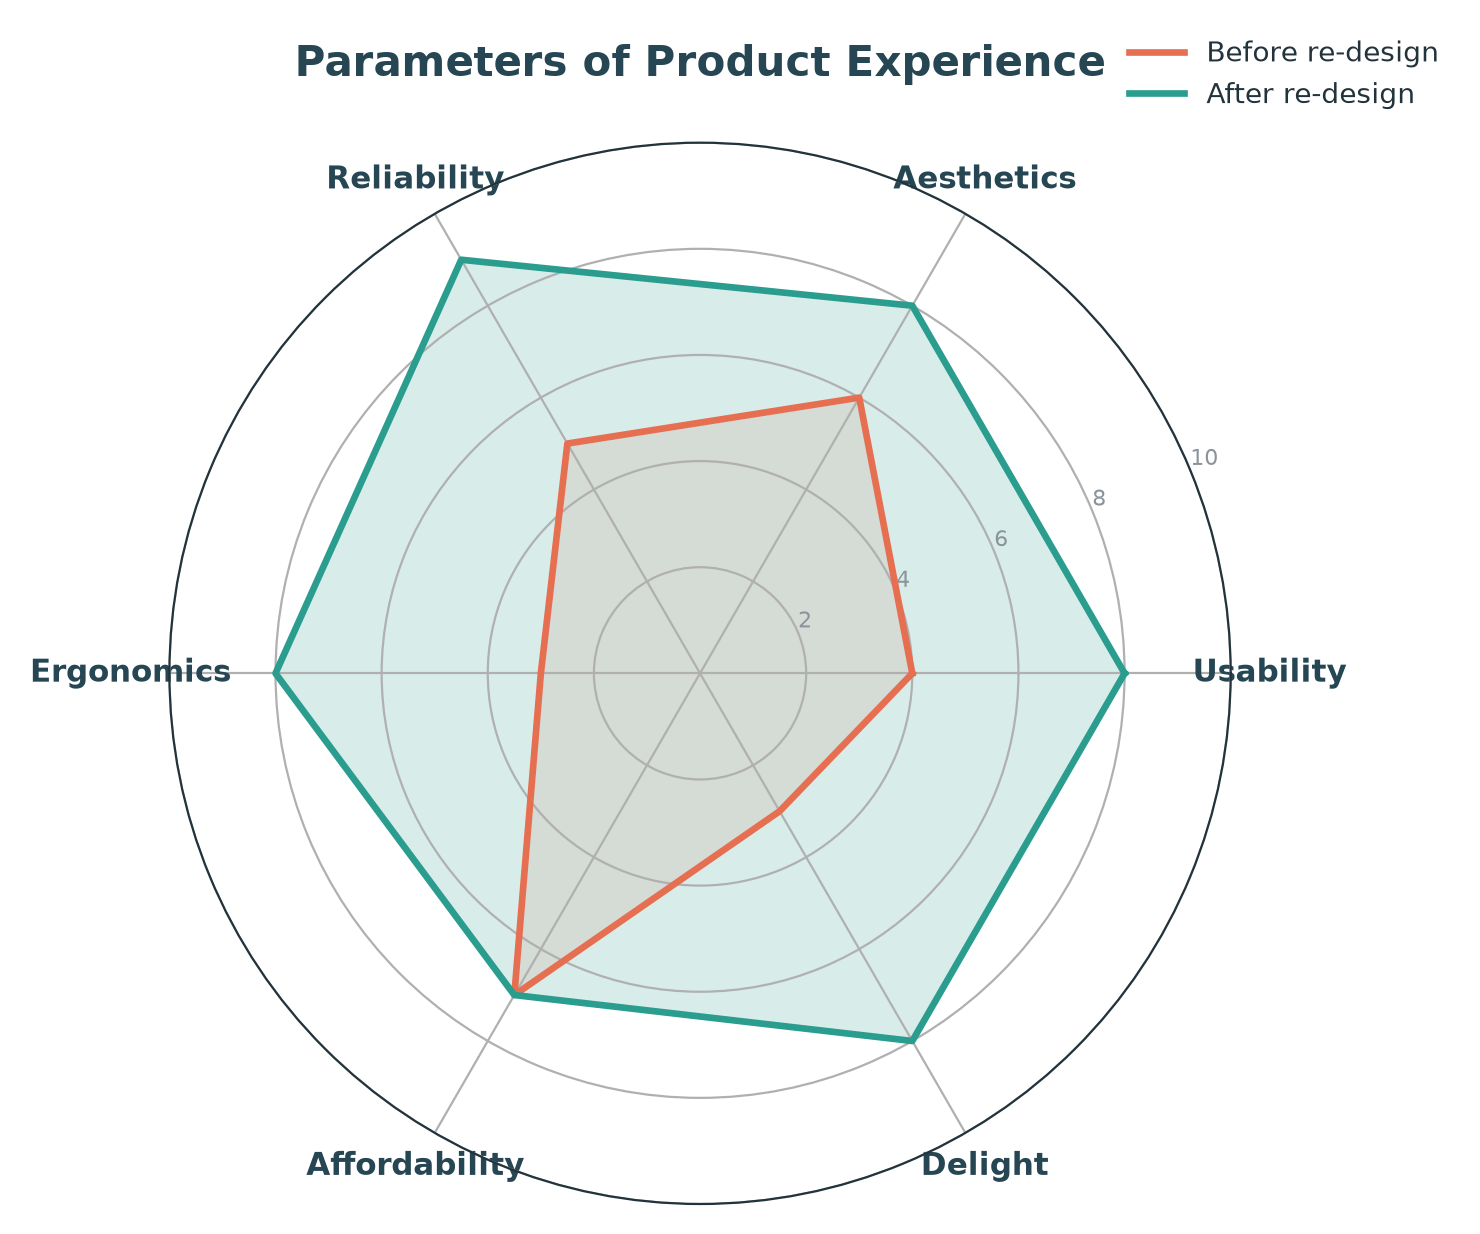
\includegraphics[width=\linewidth]{figures/cx_radar.png}
    \end{column}
    \begin{column}{0.45\textwidth}\scriptsize
      Product experience is multi-dimensional:
      \begin{itemize}\scriptsize
        \item \kwt{Usability} \& \kwt{Reliability}
        \item \kwt{Aesthetics} \& \kwt{Ergonomics}
        \item \kwt{Affordability} \& \kwt{Delight}
      \end{itemize}
      \vspace{0.3em}
      Thoughtful re-design lifts every axis — turning a merely functional
      product into one customers \emph{love}.
    \end{column}
  \end{columns}
\end{frame}

\begin{frame}{Aligning Customer Expectations}
  \begin{columns}[c]
    \begin{column}{0.55\textwidth}
      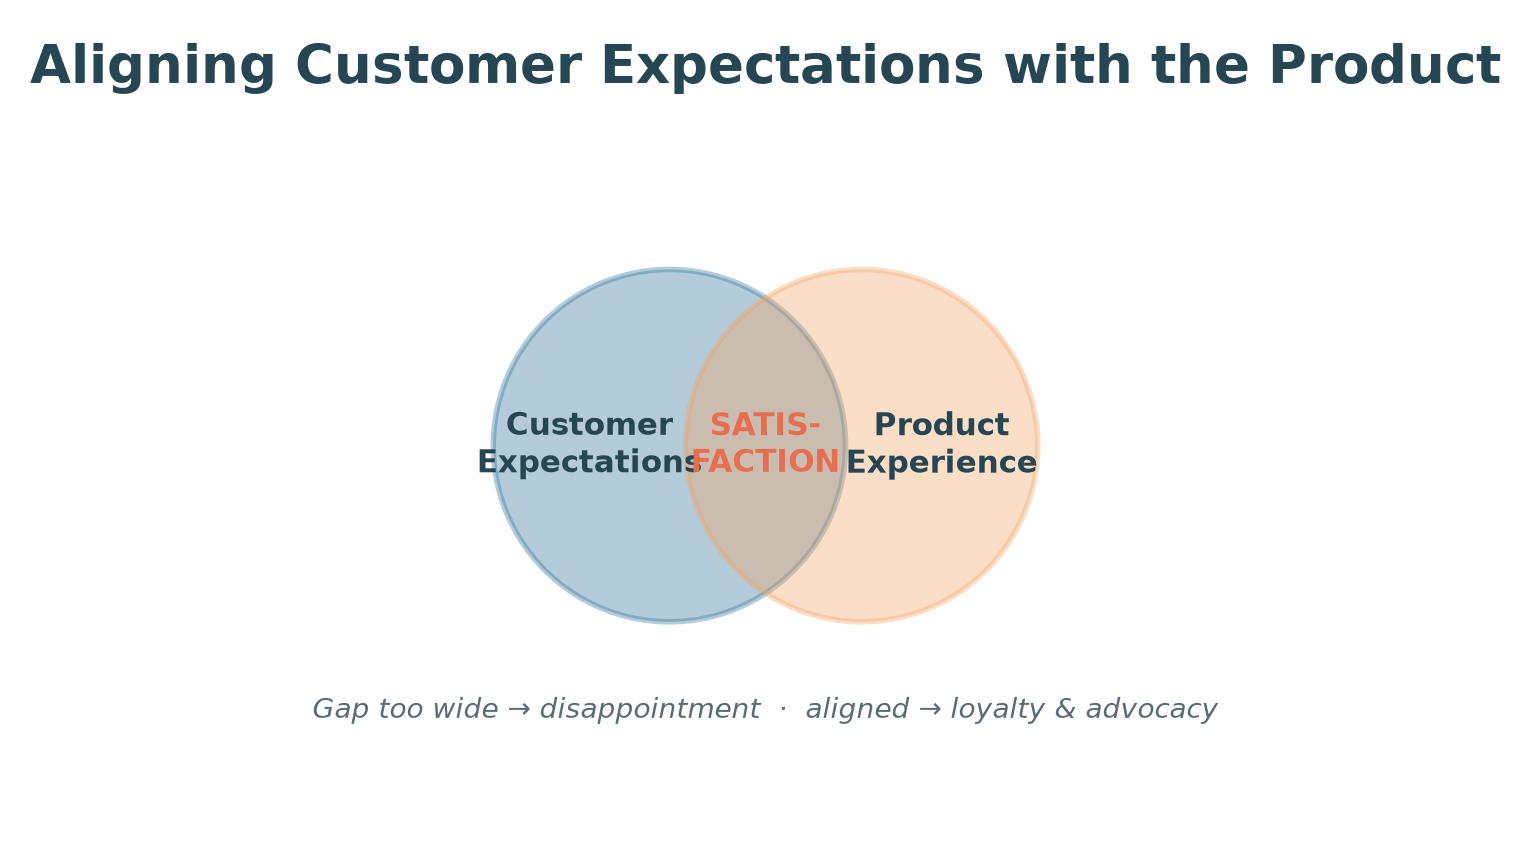
\includegraphics[width=\linewidth]{figures/expectation_alignment.png}
    \end{column}
    \begin{column}{0.45\textwidth}\scriptsize
      \kw{Satisfaction} lives where \emph{expectations} meet \emph{experience}.
      \begin{itemize}\scriptsize
        \item Gap too wide $\to$ disappointment.
        \item Well aligned $\to$ loyalty \& advocacy.
      \end{itemize}
      \vspace{0.3em}
      Manage expectations honestly \emph{and} raise the experience to close
      the gap.
    \end{column}
  \end{columns}
\end{frame}

\begin{frame}{Feedback, Re-Design \& Re-Create}
  \begin{columns}[c]
    \begin{column}{0.52\textwidth}
      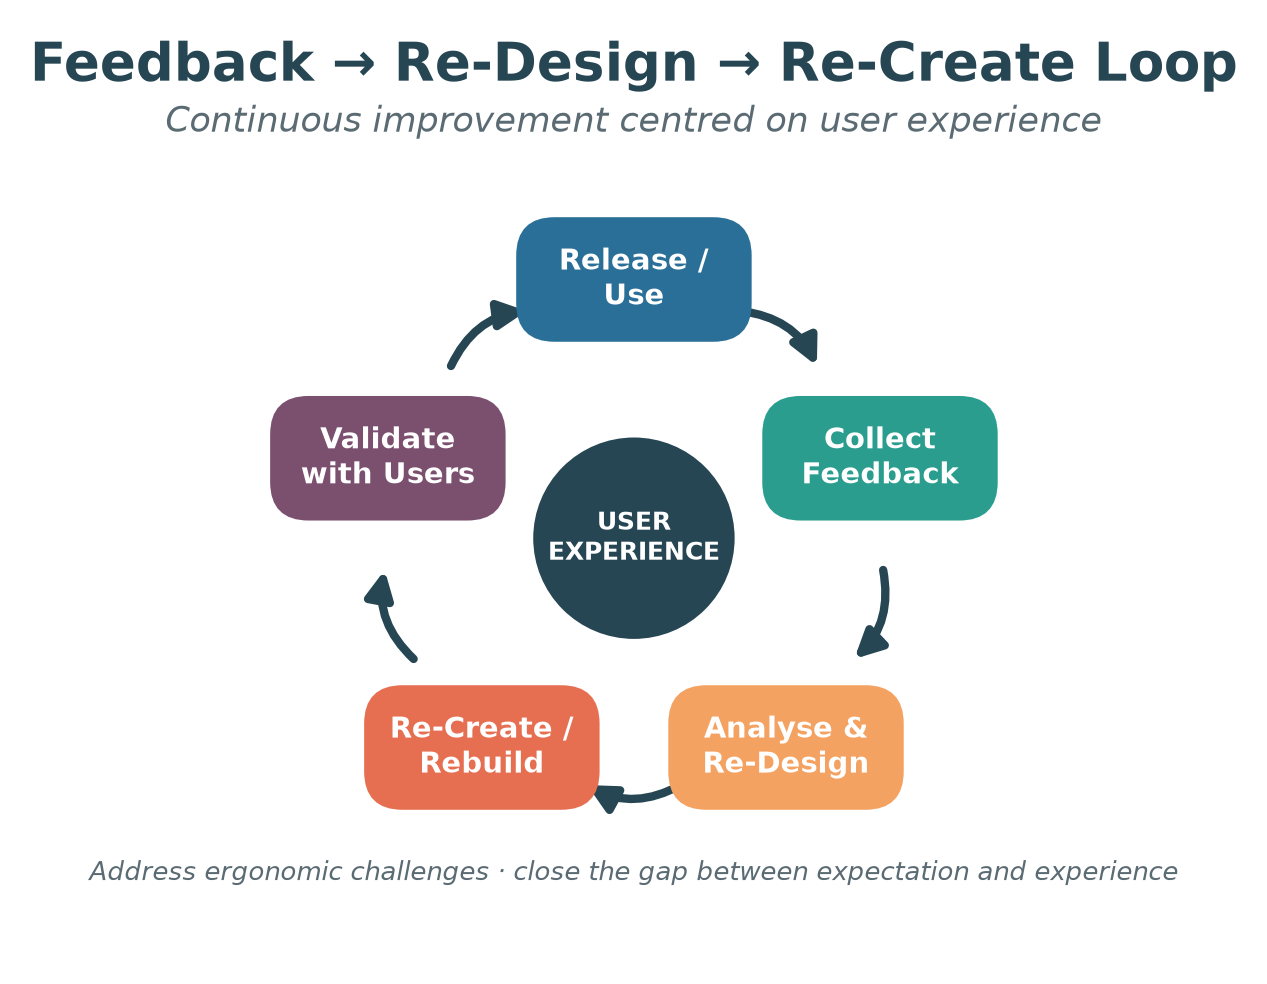
\includegraphics[width=\linewidth]{figures/feedback_loop.png}
    \end{column}
    \begin{column}{0.48\textwidth}\scriptsize
      The \kw{feedback loop} keeps a product improving:
      \begin{enumerate}\scriptsize
        \item Release \& use.
        \item Collect feedback.
        \item Analyse \& re-design.
        \item Re-create / rebuild.
        \item Validate with users.
      \end{enumerate}
      \vspace{0.2em}
      Focus relentlessly on \kwt{user experience} and address ergonomic
      challenges each cycle.
    \end{column}
  \end{columns}
\end{frame}

\begin{frame}{User-Focused Design \& the Final Product}
  \accentrule\\[0.3em]
  \begin{columns}[T]
    \begin{column}{0.5\textwidth}\small
      \textbf{User-focused design}
      \begin{itemize}\small
        \item Design \emph{with} users, not just for them.
        \item Fit the product to the human — \kwt{ergonomics}.
        \item Test with real tasks in real contexts.
      \end{itemize}
    \end{column}
    \begin{column}{0.5\textwidth}\small
      \textbf{Toward the final product}
      \begin{itemize}\small
        \item Converge feedback into refinements.
        \item Validate safety, comfort \& usability.
        \item Ship — then keep listening.
      \end{itemize}
    \end{column}
  \end{columns}
  \vspace{0.3em}
  \begin{block}{Remember}\scriptsize
    A "final" product is really the \emph{best current version} — the loop
    never truly ends.
  \end{block}
\end{frame}

%% Requires the macros/colours defined in main.tex's preamble.

%==============================================================================
\section{Design Thinking \& Customer Centricity}
%==============================================================================
\unitdivider{IV}{Design Thinking \&\\Customer Centricity}{Experience, feedback \& re-creation}

\begin{frame}{Practical Customer Challenges}
  \accentrule\\[0.3em]
  \small
  Real customers face everyday frustrations that design thinking can solve:
  \begin{columns}[T]
    \begin{column}{0.5\textwidth}
      \begin{itemize}\small
        \item Products that are \kwc{hard to assemble} or use.
        \item Confusing instructions \& interfaces.
        \item Poor \kwc{ergonomics} causing discomfort.
      \end{itemize}
    \end{column}
    \begin{column}{0.5\textwidth}
      \begin{itemize}\small
        \item Long waits and clunky service.
        \item Features nobody asked for.
        \item A gap between the \emph{promise} and the \emph{experience}.
      \end{itemize}
    \end{column}
  \end{columns}
  \vspace{0.4em}
  \begin{block}{Design thinking to the rescue}\scriptsize
    By empathising with customers we uncover these pains and re-design the
    product experience around them.
  \end{block}
\end{frame}

\begin{frame}{Parameters of Product Experience}
  \begin{columns}[c]
    \begin{column}{0.55\textwidth}
      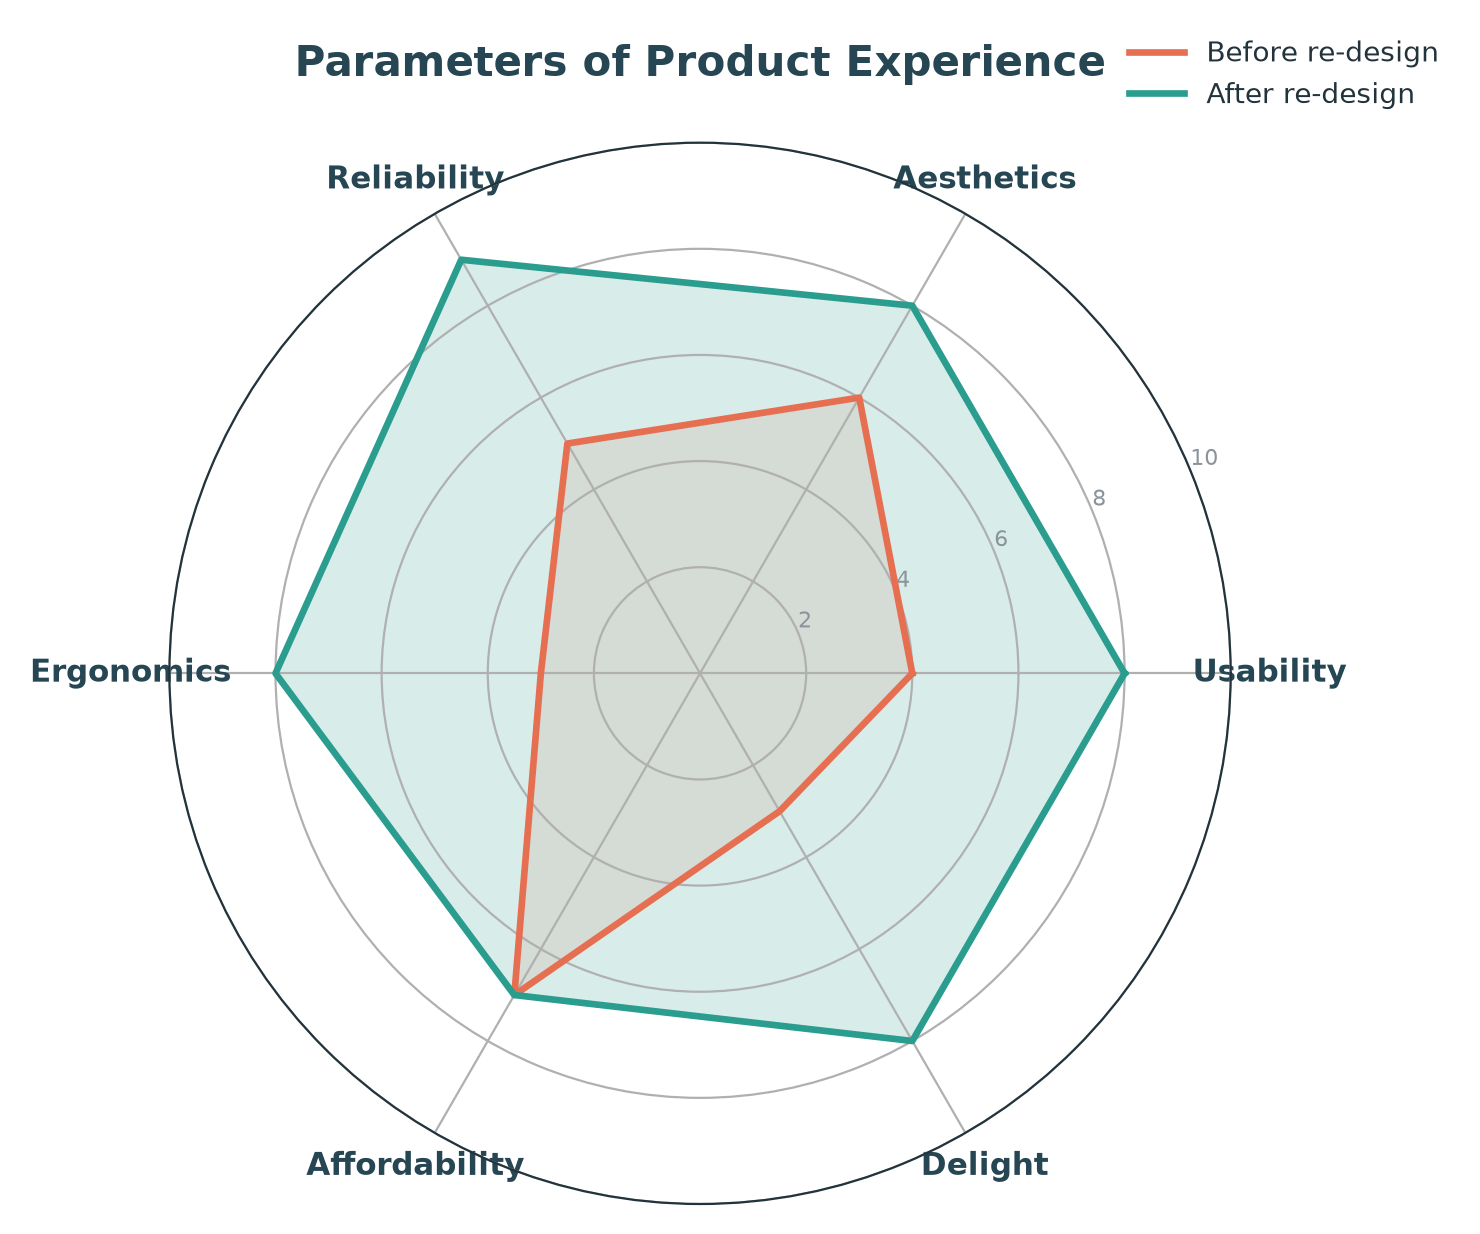
\includegraphics[width=\linewidth]{figures/cx_radar.png}
    \end{column}
    \begin{column}{0.45\textwidth}\scriptsize
      Product experience is multi-dimensional:
      \begin{itemize}\scriptsize
        \item \kwt{Usability} \& \kwt{Reliability}
        \item \kwt{Aesthetics} \& \kwt{Ergonomics}
        \item \kwt{Affordability} \& \kwt{Delight}
      \end{itemize}
      \vspace{0.3em}
      Thoughtful re-design lifts every axis — turning a merely functional
      product into one customers \emph{love}.
    \end{column}
  \end{columns}
\end{frame}

\begin{frame}{Aligning Customer Expectations}
  \begin{columns}[c]
    \begin{column}{0.55\textwidth}
      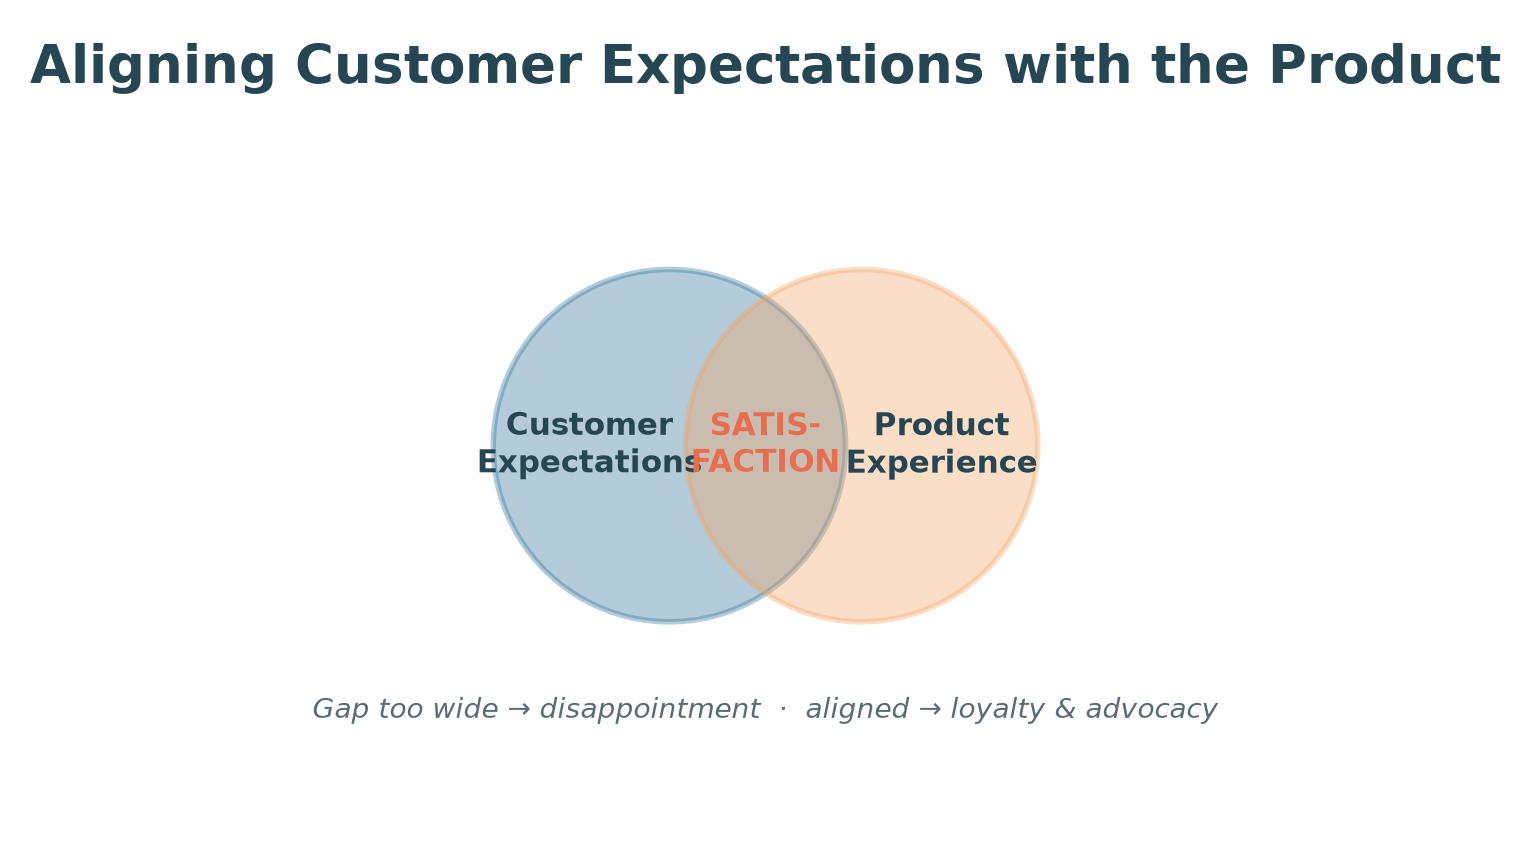
\includegraphics[width=\linewidth]{figures/expectation_alignment.png}
    \end{column}
    \begin{column}{0.45\textwidth}\scriptsize
      \kw{Satisfaction} lives where \emph{expectations} meet \emph{experience}.
      \begin{itemize}\scriptsize
        \item Gap too wide $\to$ disappointment.
        \item Well aligned $\to$ loyalty \& advocacy.
      \end{itemize}
      \vspace{0.3em}
      Manage expectations honestly \emph{and} raise the experience to close
      the gap.
    \end{column}
  \end{columns}
\end{frame}

\begin{frame}{Feedback, Re-Design \& Re-Create}
  \begin{columns}[c]
    \begin{column}{0.52\textwidth}
      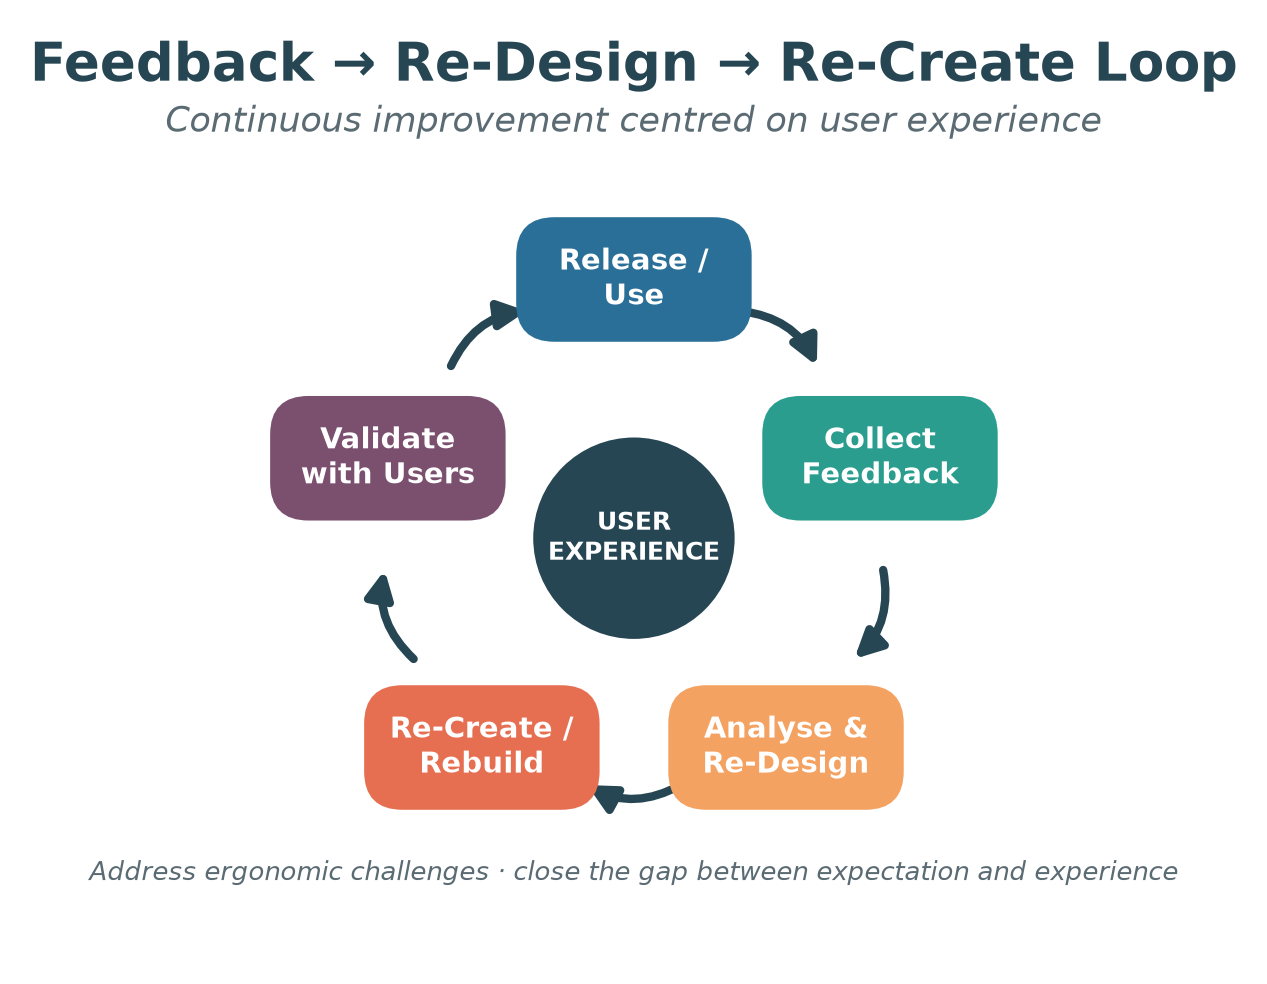
\includegraphics[width=\linewidth]{figures/feedback_loop.png}
    \end{column}
    \begin{column}{0.48\textwidth}\scriptsize
      The \kw{feedback loop} keeps a product improving:
      \begin{enumerate}\scriptsize
        \item Release \& use.
        \item Collect feedback.
        \item Analyse \& re-design.
        \item Re-create / rebuild.
        \item Validate with users.
      \end{enumerate}
      \vspace{0.2em}
      Focus relentlessly on \kwt{user experience} and address ergonomic
      challenges each cycle.
    \end{column}
  \end{columns}
\end{frame}

\begin{frame}{User-Focused Design \& the Final Product}
  \accentrule\\[0.3em]
  \begin{columns}[T]
    \begin{column}{0.5\textwidth}\small
      \textbf{User-focused design}
      \begin{itemize}\small
        \item Design \emph{with} users, not just for them.
        \item Fit the product to the human — \kwt{ergonomics}.
        \item Test with real tasks in real contexts.
      \end{itemize}
    \end{column}
    \begin{column}{0.5\textwidth}\small
      \textbf{Toward the final product}
      \begin{itemize}\small
        \item Converge feedback into refinements.
        \item Validate safety, comfort \& usability.
        \item Ship — then keep listening.
      \end{itemize}
    \end{column}
  \end{columns}
  \vspace{0.3em}
  \begin{block}{Remember}\scriptsize
    A "final" product is really the \emph{best current version} — the loop
    never truly ends.
  \end{block}
\end{frame}
